\section{Results} \label{sec:results}
For our experiments with synthetic data, 


Once the trees had been rooted, a general linear model with the normal family was constructed with the with expected number of substitutions as the input, and sampling time as the response. 
For all experiments using patient data, this fit was only over the plasma data, and the PBMCs expected subs were used as input. 
From this, we collected the difference between the observed sampling date, and the predicted date. 

In all of our experiments, before any analysis is done, all times are re-scaled to lie between $0$ and $1$. 
This is calculated as $ \text{new time} = \frac{\text{time} - \text{min\_time}}{\text{max\_time} - \text{min\_time}}$, this gives normalized time. 
Errors are then calculated from this number.

\begin{figure*}[!ht] \label{fig:results1}
	\centering
	\includegraphics[trim=0cm 0cm 0cm 6cm, clip=true, scale=0.425]{figures/simulated.pdf} \\
	\includegraphics[trim=0cm 0cm 0cm 7cm, clip=true,scale=0.425]{figures/simulated_latent.pdf}\\
	\includegraphics[trim=0cm 0cm 0cm 7cm, clip=true,scale=0.425]{figures/ancre.pdf}\\
	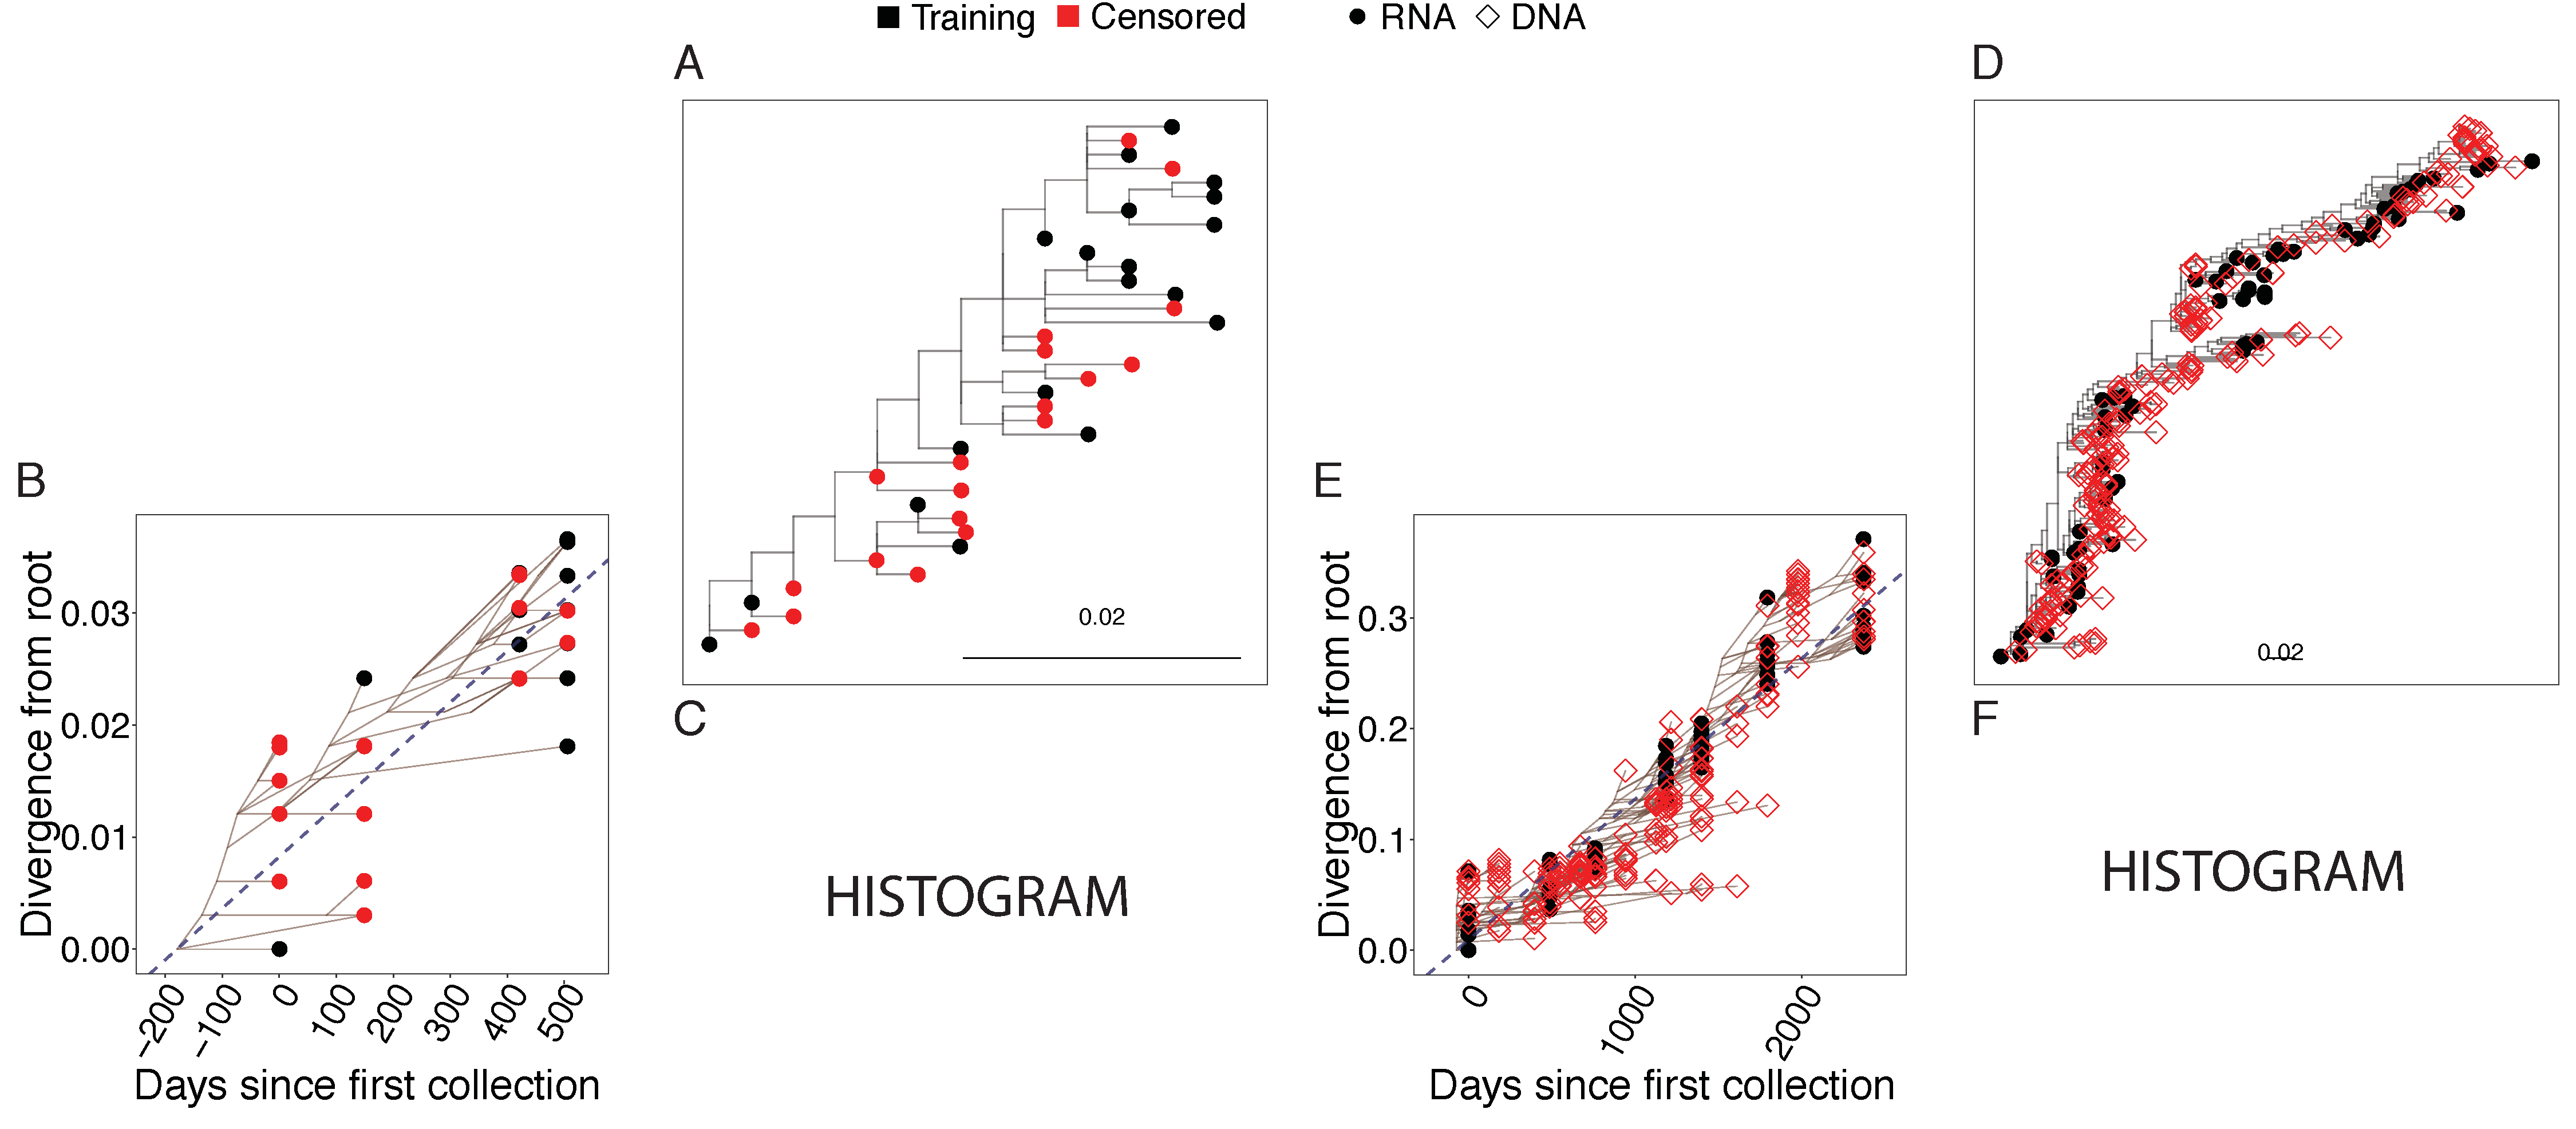
\includegraphics[trim=0cm 4cm 0cm 7cm, clip=true,scale=0.425]{figures/lanl.pdf}
	\caption[Examples]{\anote{Add legend, change points, change shading, explain point colouring, explain mean and median lines.}}
\end{figure*}


\subsection{Simulated Data} \label{sec:sim_results}
For our simulated data, we evaluated two error metrics. 
We look at the mean square error for each individual, as well as the mean, and median error. 
Unsurprisingly the error for this is really low because the phylogeny is clocklike and very informative. 
Also, in figure whatever there'��s a set of superimposed density estimates of the error. 
Each image in it represents one run (look at a tree and remove up to 50\% of the samples in that tree). 
For the simulated latent data, the normalized error is higher in all cases, also the density estimates are shifted in towards the right, indicating that the latent behaviour has an effect on the reconstruction, also there’s more variation in the plots.


\subsection{RNA Only Data} \label{sec:rna_only}
For our reconstruction of RNA only data, they pretty much mimicked the simulated data. 
Except we had a higher mean RMS. 
This is all not surprising because of natural variation.  

\subsection{Patient Reconstruction}
Qualitatively many plots show examples of latency, quantitavely it's difficult to say. 

